\section{Process description, problem definition and modelling}

In this section the process of a wind turbine generating electricity is examined.
Fragoso et~al. analyse a lab-scale model of wind turbine with regard to decoupling control and multivariable robust control \cite{Fragoso_et_al_2017}.
The section starts with a brief introduction of the process, then analyses the control design aspects and summarizes with the model equations and further reading material.

\subsection{Introduction and process description}

% Introduction
According to the International Energy Agency (IEA), the renewable electricity generation worldwide by wind has gone up from \SI{342205.0}{\GW\hour} in 2010 to \SI{1598080.0}{\GW\hour} in 2020 \cite{IEA_renewables_wind_world_2022}. 
Looking at Germany the same trend can be seen by IEA: From \SI{38547.0}{\GW} in 2010 to  \SI{113848.0}{\GW\hour} in 2020. 
By comparing this with solar PV (\SI{11729.0}{\GW\hour} in 2010 to \SI{49992.0}{\GW\hour} in Germany), the huge increase becomes clear \cite{IEA_renewables_wind_world_2022}. 

% Description
The system by Fragoso et~al. consists of a lab-sized rotor with two blades and a permanent magnet DC electric generator placed inside a wind tunnel \cite{Fragoso_et_al_2017}.
This system is decomposed into two subsystems: First the mechanical subsystem describing the rotor and second the electrical subsystem describing the generator.
The system equations for both subsystems are derived and a linear model is developed.
To better understand the coupling of system states the relative gain array is analysed.
In the second half, different tools for controller design are discussed and later simulation data is compared with experimental data.

For defining a control objective it is necessary to know the four operating condition with respect to wind speed: (1) cut-in, (2) partial load, (3) transition,  (4) full load and (5) cut-out.
Partial and full load are the two status of most interest.
Transition describes the pass from operating state (2) to (4).
While cut-in and cut-out are the state with too little and too much wind to operate the turbine.


\subsection{Control design aspects}

\begin{figure}[h]
    \center
    \subcaptionbox{Process diagram of a windturbine \cite{Simani_2015}. \label{fig:process_diagram}}[.45\textwidth]{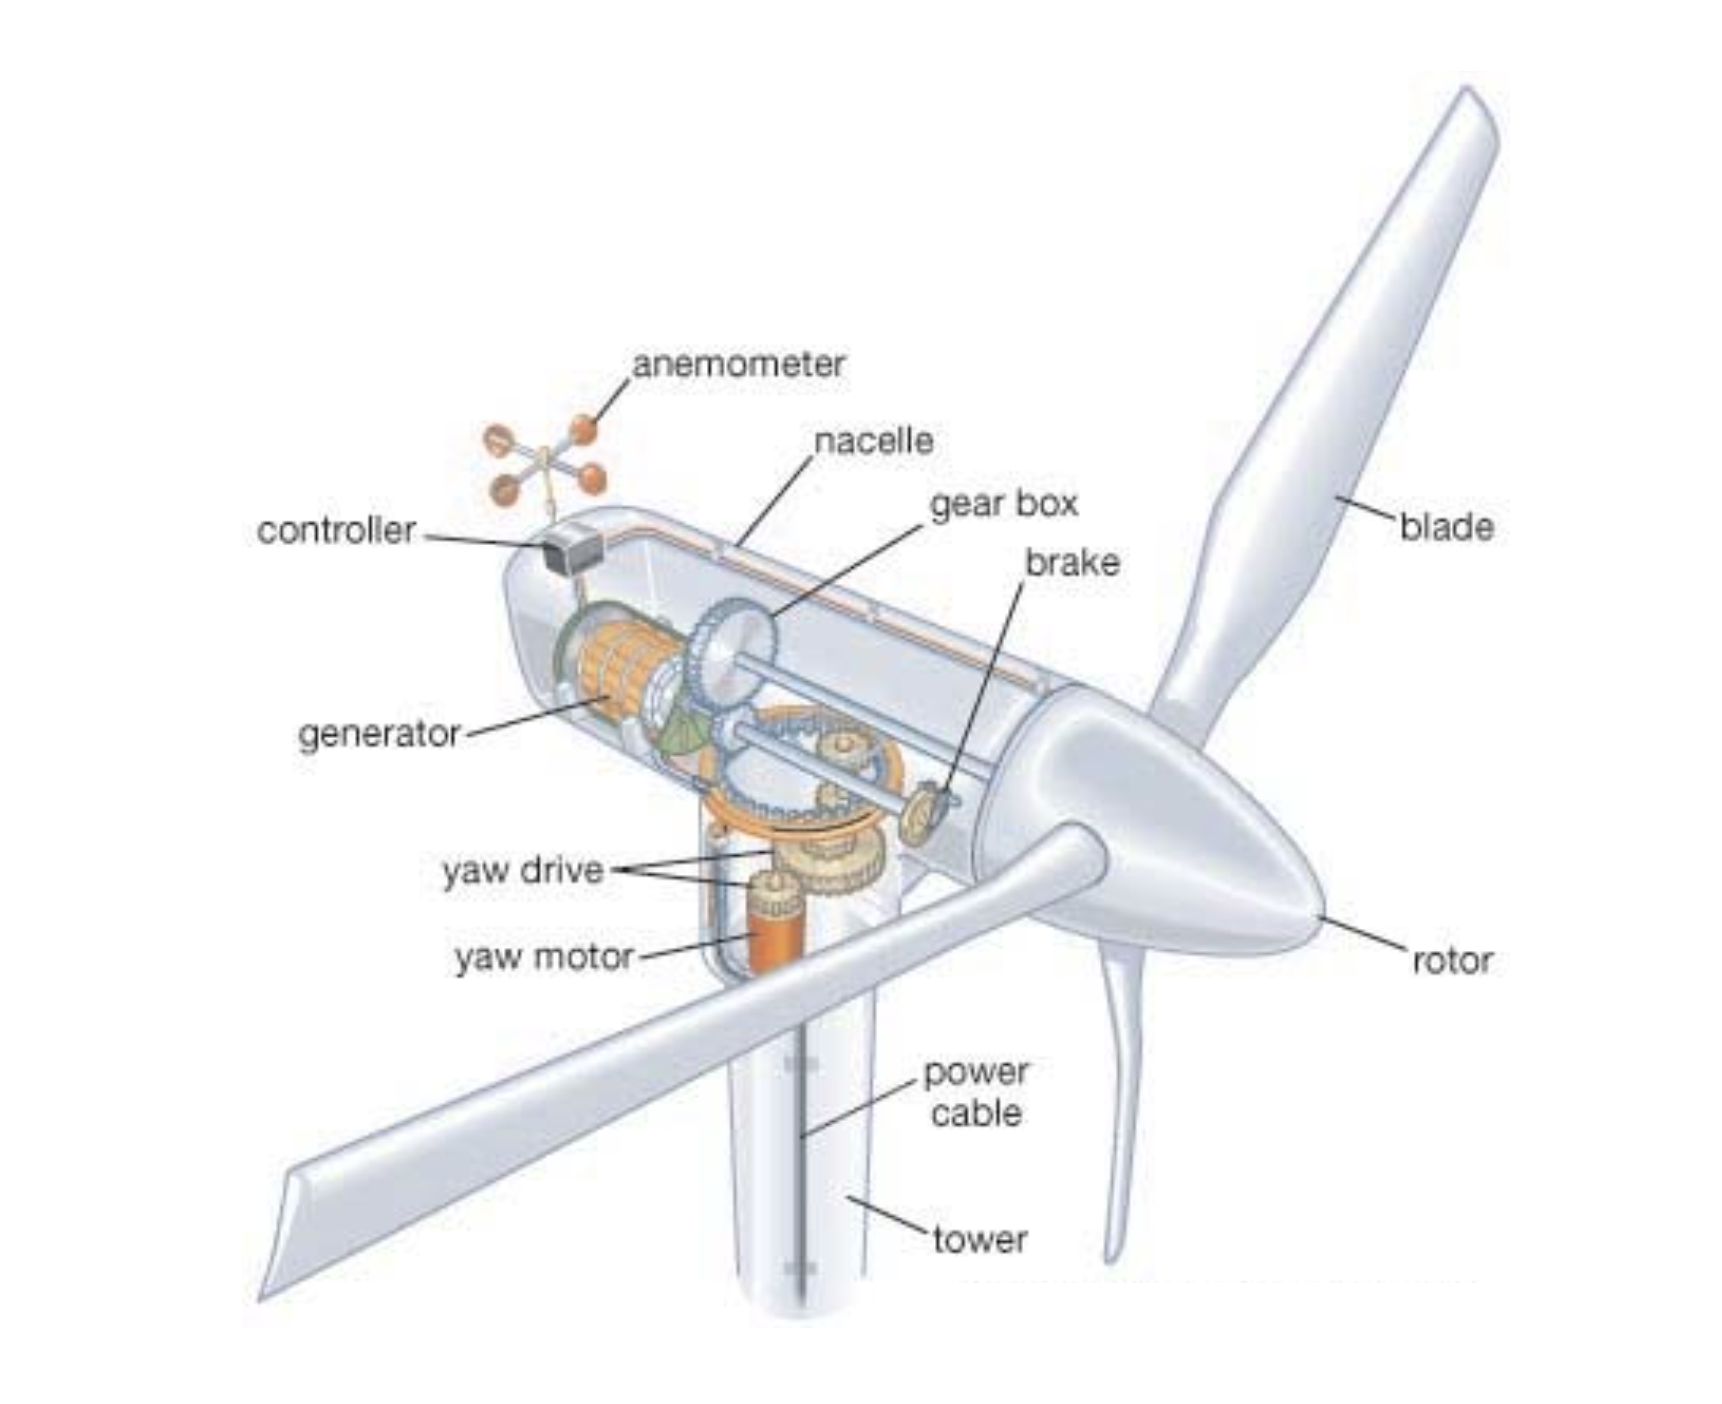
\includegraphics[width=1\linewidth]{fig/Simani_2015_process_diagram.png}}
%    
    \subcaptionbox{Control block diagram of a a wind turbine model \cite{Fragoso_et_al_2017}. Consisting of the input variables (left), the output variables (right), the controller (Multivariable control), the wind turbine itself and the wind as a disturbance. \label{fig:control_block_diagram} }[.45\textwidth]{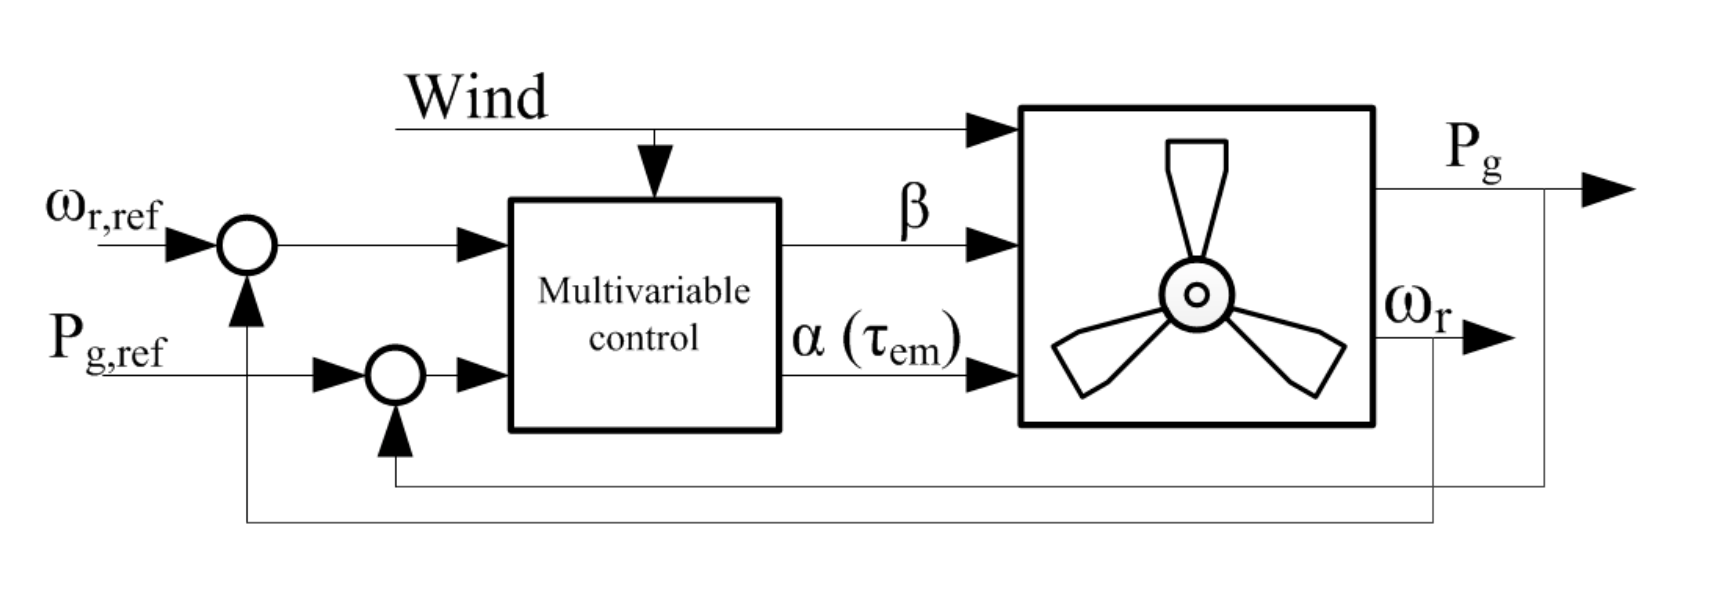
\includegraphics[width=1\linewidth]{fig/Fragaso_et_al_2017_process_scheme.png}}
%
    \caption{Comparison of a process diagram and the control block representation of a wind turbine.}
    \label{fig:compare_block_diagram_vs_process_diagram}
\end{figure}

\textbf{Control objective} Fragoso et~al. discusing two different objective at two different operating states.
If the turbine is operated in partial load the objective is to maximize the power that can be captured from the wind.
The objective changes to maintaining the power constant at the rated power if the turbine is operated in full load.

\textbf{Input variables} Pitch angle $\beta$ and generator torque $\tau_{em}$ are commonly used as input variables. 

\textbf{Output variables} The rotational speed $\omega_r$ and generated electric power $P_G$ are the output variables of the system.

\textbf{Constraints} For controller design a linear model (derived by identification) is obtained by the authors. 
For further constraints Figure 13 and Figure 14 in Fragoso et~al. publications are analyzed.
The following constraints can be seen in the output and control signals.

\begin{table}[H]
    \label{tab:constraints}
    \caption{Possible constraints for input and output variables.}
    \centering
    \begin{tabular}{ccccc} \toprule
            & $\omega_r \left[\text{rpm}\right]$ & $P_G \left[\si{\watt}\right]$ & $\beta \left[\si{\degree}\right]$ & $\alpha \left[\text{\%}\right]$ \\ \midrule
        Min & 1550 & 5 & 0  & 60 \\
        Max & 1750 & 7 & 25 & 75 \\ \bottomrule
    \end{tabular}
\end{table}


\textbf{Operating characteristics} The process is a continuous batch process.
The wind mill produces a laminar flow of air.
This is not the case in general.
If the stream of air is not laminar turbulences will occur at the blades.
This will introduces further disturbances which hard to calculate or estimate.

\textbf{Control structure}
The rotational speed $\omega_R$ and generated electric power $P_G$ are the controlled variables, blade pitch angle $\beta$ and the duty cycle $\alpha$ are the manipulated variables and the wind speed $v$ is counted as a disturbance.
The system is a multiple input multiple output (MIMO) system or two input and two output (TITO) system.
In total one $\text{H}_{\infty}$ based robust controller and three decoupling approaches are developed. 

\subsection{Model equation} \label{sec:intro:model_eq}

Fragoso et~al. defining their model through nonlinear ordinary differential equations. They distinguish between the electromechanical and electrical subsystems. Here only a brief overview is given. All relevant equations and parameter are published \cite{Fragoso_et_al_2017}.

For the mechanical subsystem the rotational speed $\omega_R$ is given by
\begin{align}
    J_t \frac{d\omega_r}{dt} = \tau_a - \tau_{em}
\end{align}
Here $J_t$ is the total inertia momentum of the system.
$\tau_{em}$ is the electromechanical torque and $ \tau_a$ the aerodynamic torque which can be expressed as a nonlinear function of wind speed $v$ and a power coefficient $C_p(\lambda ,\beta)$.
Where $\lambda$ is the tip speed ratio and $\beta$ the pitch angle.
Fragoso et~al. especially describe the power coefficient as an important parameter for the control and emphasises its nonlinear influence to the systems dynamics.


The electromechanical torque and the generated electrical power define the electrical subsystem.
\begin{align}
    \tau_{em} &= k_t i_g \label{eq:intro:tau_em}\\
    P_g &= \eta \tau_{em} \omega_r \label{eq:intro:P_g}
\end{align}
In both equations the efficiency is represented by $k_t$ and $\eta$ respectively for the electromechanical torque and the generator.


\subsection{Further reading}

\begin{figure}[htp]
    \centering

    \subcaptionbox{Process block diagram of a wind turbine with dynamics of field current and blade angles \cite{Adanez_et_al_2018}. \label{fig:Adanez_turbine_scheme}}[.3\textwidth]{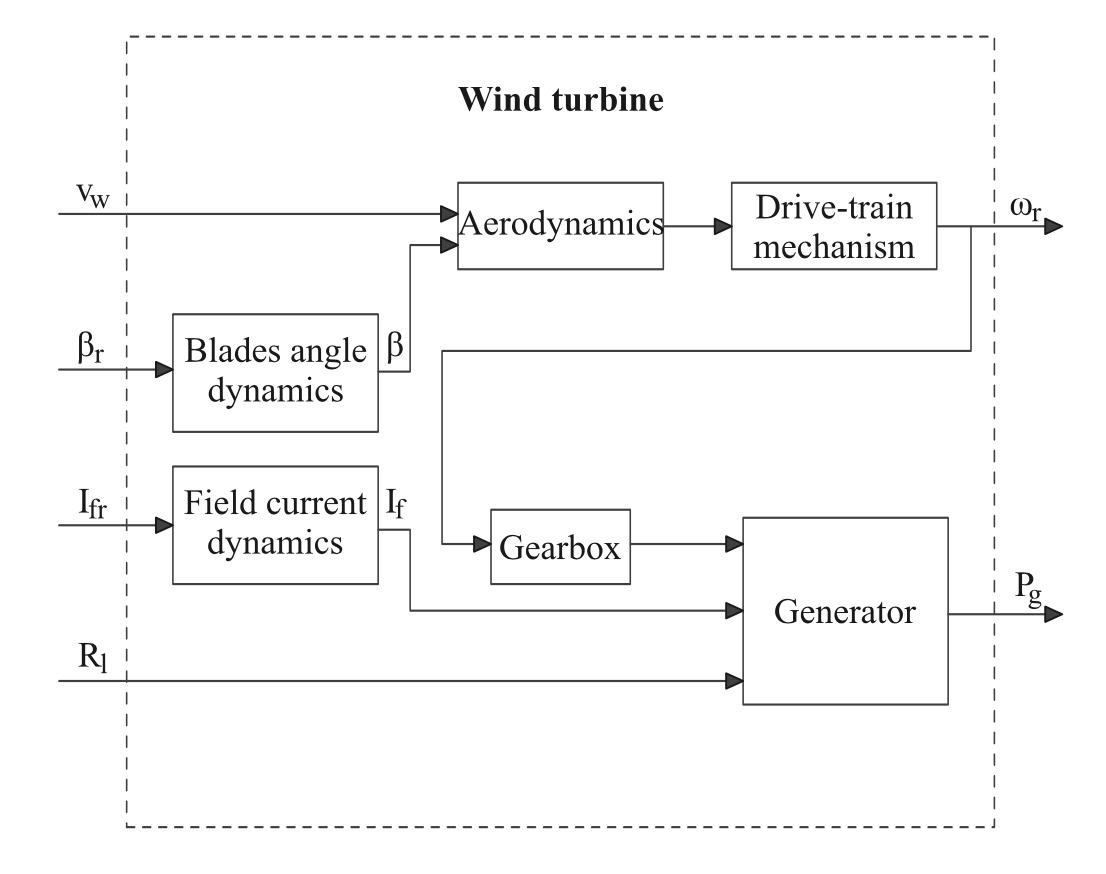
\includegraphics[width=1\linewidth]{fig/Adanez_et_al_2018_turbine_scheme.png}}
%
    \subcaptionbox{The control scheme used by Yuan, Cheng and Tang \cite{Yuan_Chen_Tang_2020}.  \label{fig:Yuan_Chen_Tang_control_scheme}}[.3\textwidth]{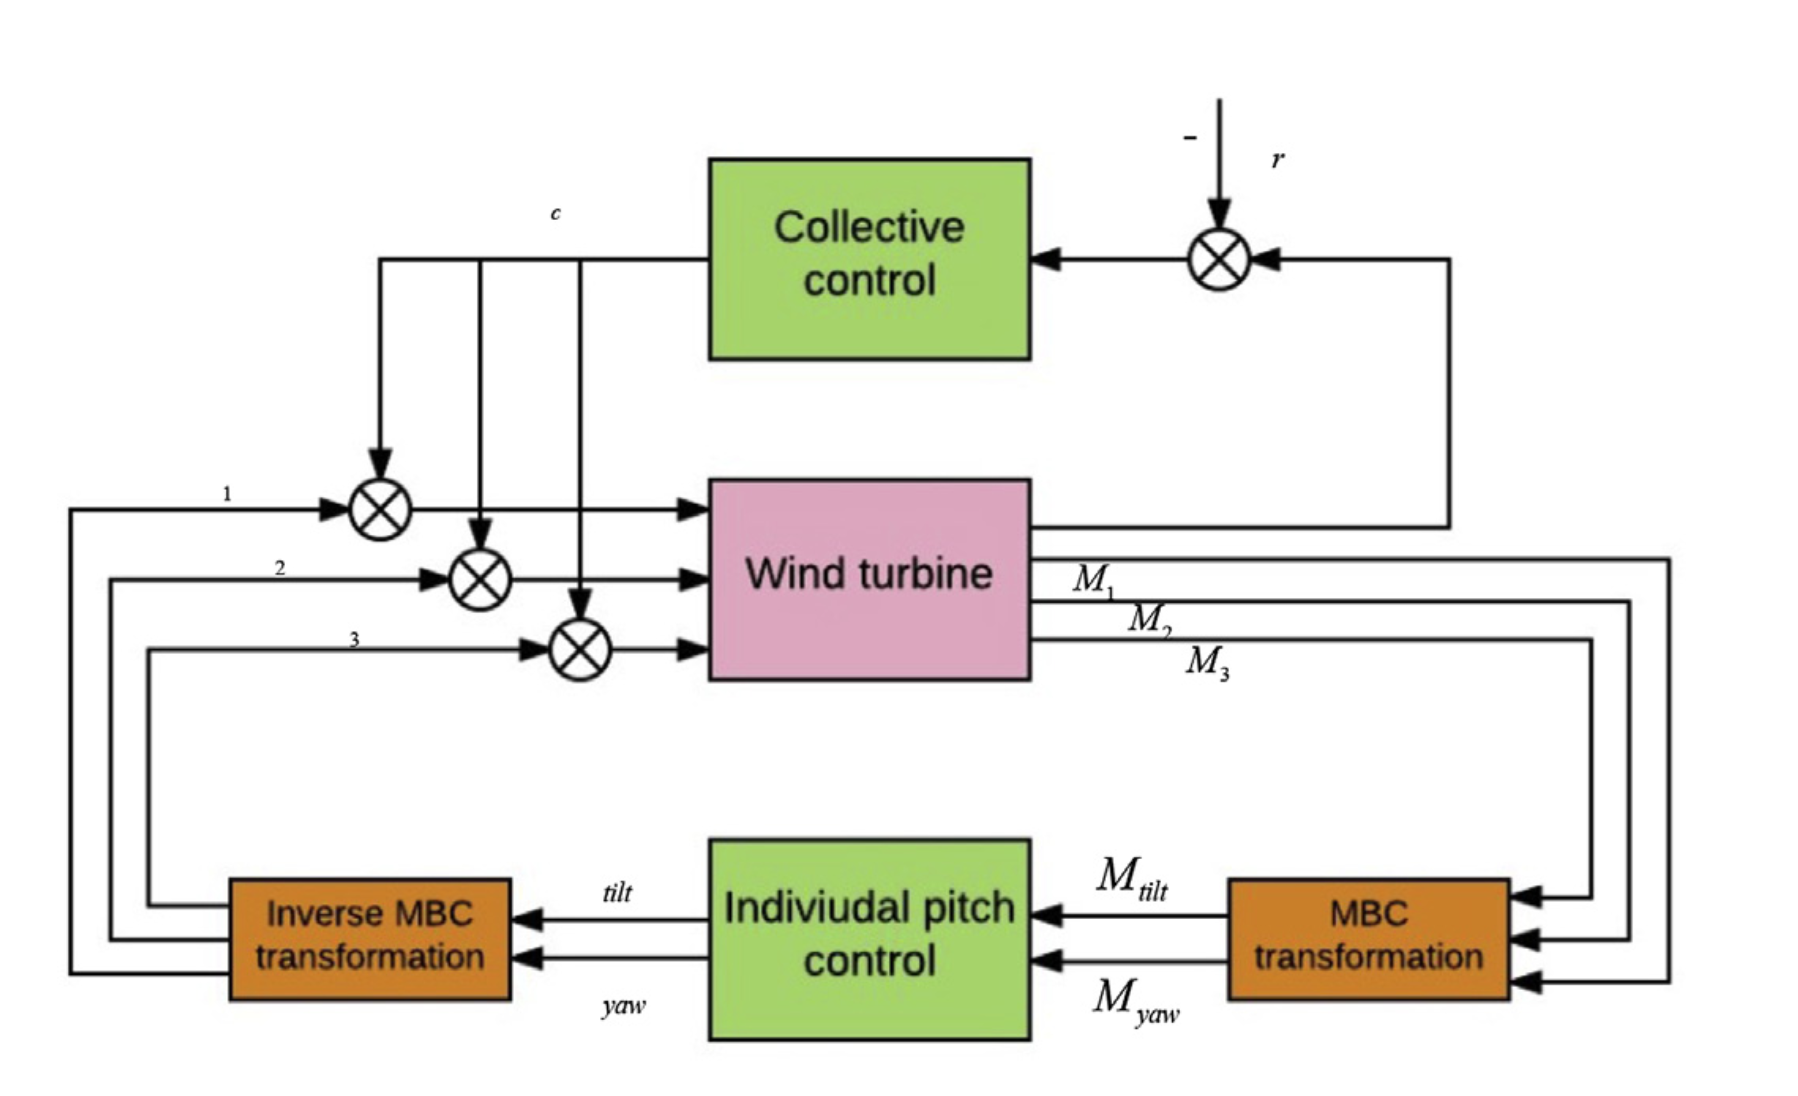
\includegraphics[width=1\linewidth]{fig/Yuan_Chen_Tang_2020_advanded_control.png}}
%
    \subcaptionbox{Visualization of switching control structures when wind turbine is in different operating conditions \cite{Simani_2015}.  \label{fig:Simani:switching_control}}[.3\textwidth]{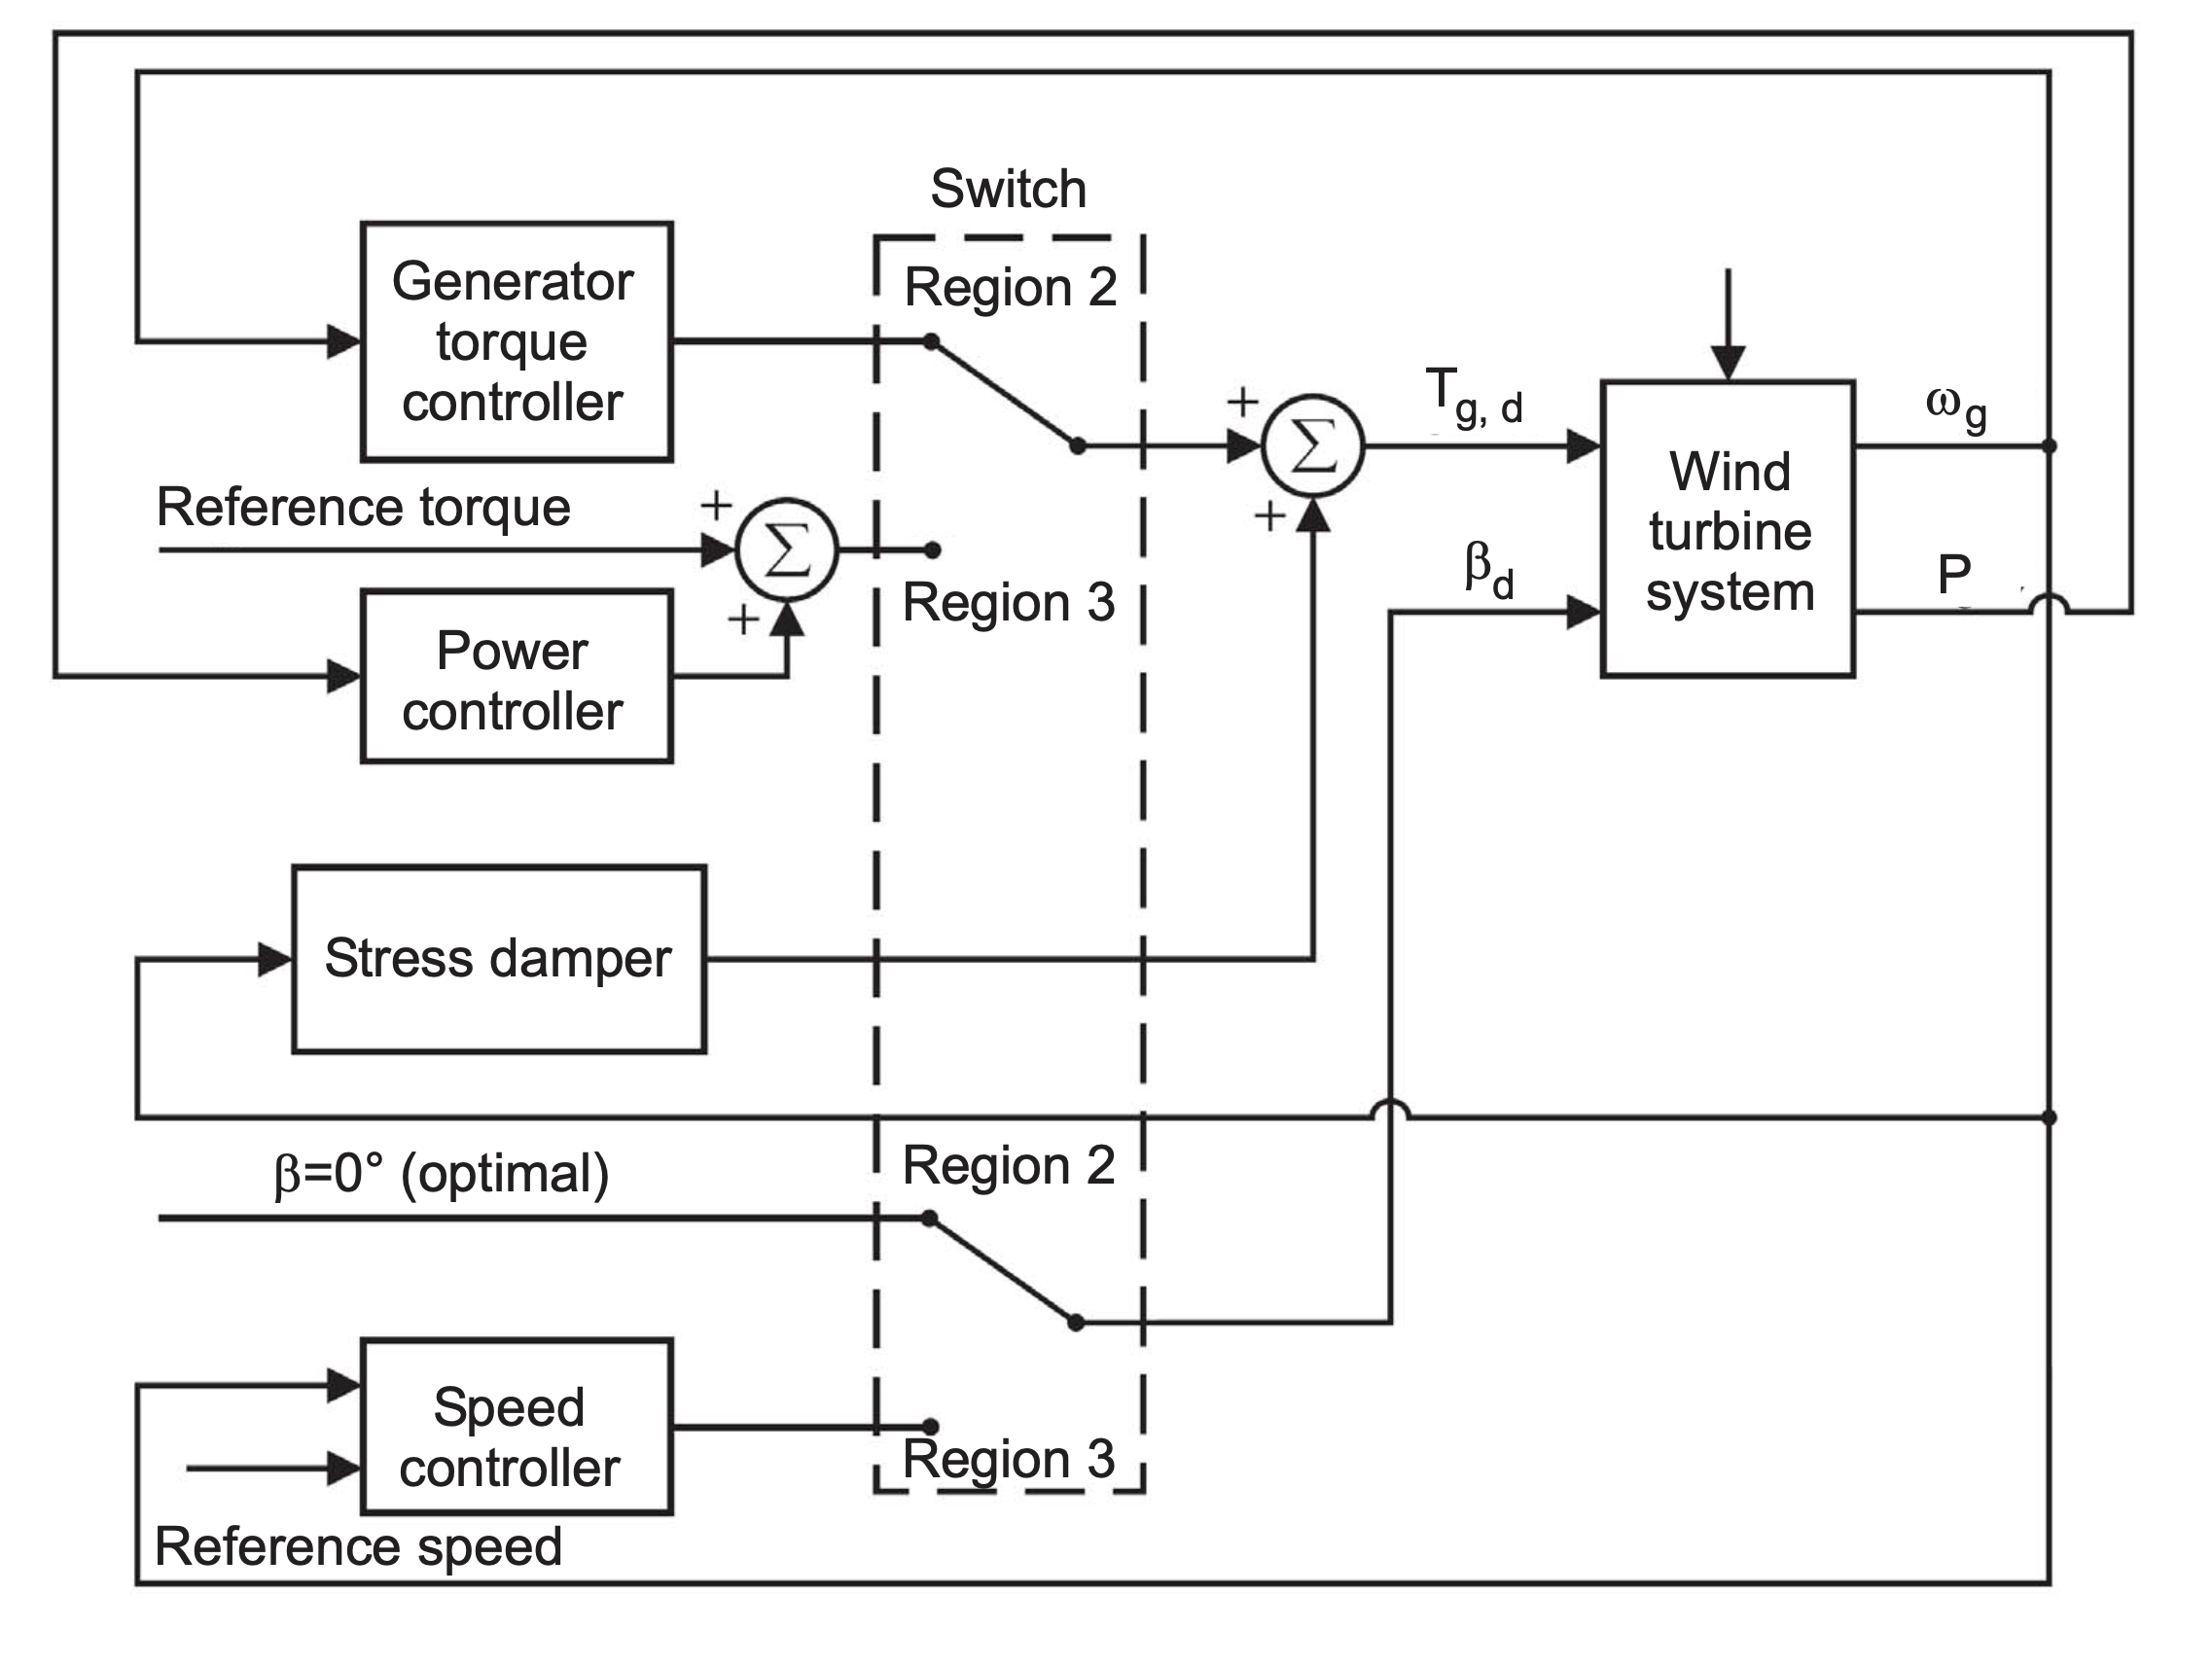
\includegraphics[width=1\linewidth]{fig/Simani_2015_switching_control.png}}
%
    \caption{Comparison of different visualization of control and system structures.}
    \label{fig:different_schemes_compared}
\end{figure}

Adánez et~al. published a control approach for a wind turbine based on incremental state model in 2018 \cite{Adanez_et_al_2018}.
The authors gave an overview over recent literature before describing their model of a wind turbine.
In comparison to Fragoso et~al. their schematics showing a more detailed look at the different parts of the system (\autoref{fig:Adanez_turbine_scheme}).
At the same time, however, it can be seen that very similar input and output variables are used.
They develope a multivariable discrete state model and an incremental state model. Besides that, an observer for the state feedback controller is derived.



Yuan, Cheng and Tang are describing in their work from 2020 the problems arising from the increasing blade sizes of modern wind turbines and thereby developing challenges in controller design \cite{Yuan_Chen_Tang_2020}.
In contrast to the aforementioned publication the authors do not show a scheme of the overall system, but instead providing a visual representation of the control structure (\autoref{fig:Yuan_Chen_Tang_control_scheme}).
The system itself is implemented in third party code and not as clearly shown as in the other publications.

Simani gives an full overview of the topic of modeling wind turbines \cite{Simani_2015}.
He summarizing not only models for the generator and blades but also for the wind turbine tower itself and the dynamics regarding blade motions.
In contrast to all other mentioned publication he is giving an overview of switching control structure when the turbine is in different operating conditions (\autoref{fig:Simani:switching_control}).
Also he is emphasising the switch in control objectives in different operating conditions.

\subsection{Summary}

The work of Fragoso et~al. seems to fit best in the criteria of the course by clearly naming all important design aspects and deriving comprehensible and probably easy to re-implement model.

\subsubsection{Simulating the model}

In Table 2 Fragoso et~al. published several transfer function for different wind speed.
These transfer function could be used to simulate the model.

For the ordinary differential equation all the  necessary parameters for a simulation seem to be given.
Also initial condition are formulated or could be read from Figure 13 and 14.